%%%%%%%%%%%%%%%%%%%%%%%%
% SNOPT Windows Compile Instructions
%%%%%%%%%%%%%%%%%%%%%%%%

\subsubsection{Dependency Installation Instructions}
The EMTG repository comes with sets of SNOPT CMake files for compilation of SNOPT in Windows. The following steps walk through the SNOPT compilation process using CMake.
\begin{enumerate}
	
	\item Navigate to the \textbf{\textless EMTG\_root\_dir\textgreater}\verb|\SNOPT\| directory.
	\item Copy the \verb|CMakeLists__SNOPT7-7.txt| file appropriate for your version of SNOPT and paste it into the \textbf{\textless SNOPT\_root\_dir\textgreater} directory changing the name of the file to \verb|CMakeLists.txt|.
	
	\item Navigate to the \textbf{\textless EMTG\_root\_dir\textgreater}\verb|\SNOPT\src\| directory.
	\item Copy the \verb|CMakeLists_SNOPT7-7.txt| file appropriate for your version of SNOPT and paste it into the \textbf{\textless SNOPT\_root\_dir\textgreater}\verb|\src\| directory changing the name of the file to \verb|CMakeLists.txt|.

	\item Open the \textbf{\textless SNOPT\_root\_dir\textgreater}\verb|\src\sn87sopt.f| file in a text editor
		\begin{enumerate}
			\item Navigate to approximately line 2791 for SNOPT 7.7 (line 2709 in SNOPT 7.6) and comment (Fortran uses the ! character for comments) out the line that reads 
				\begin{verbatim}
					primalInf = primalInf/max(xNorm , one)
				\end{verbatim}
			\emph{Leaving this line uncommented can incorrectly mark certain solutions as feasible in \ac{SNOPT}.}
			\item Save and close the file
		\end{enumerate}
	\item \emph{SKIP THIS STEP FOR SNOPT 7.7. This change is only required for SNOPT 7.6}\\ Open the \textbf{\textless SNOPT\_root\_dir\textgreater}\verb|\src\sn70nobj.f| file in a text editor.
		\begin{enumerate}
			\item Navigate to approximately line 235
			\item Replace the following line ...
				\begin{verbatim}
					call dload ( nF, zero, Elem, 1 )
				\end{verbatim}
				... with ...
				\begin{verbatim}
					call iload ( nF, 0, Elem, 1 )
				\end{verbatim}
				\emph{The original line could cause an error when attempting to build \ac{SNOPT} in Windows using the MinGW console as opposed to using the CMake and Visual Studio method.} 
			\item Save and close the file
		\end{enumerate}

    \item Ensure the Windows Path environment variable contains the path to the MinGW bin directory and save changes. 
	\emph{It is recommended that this be placed at or near the top of the list of directories in path. Refer to the MinGW section for additional detail.}

    \item Open the CMake GUI
	\item Set “Where is the source code” to the \textbf{\textless SNOPT\_root\_dir\textgreater} directory
	\item Set “Where to build the binaries” to \textbf{\textless SNOPT\_root\_dir\textgreater}\textbackslash build\textbackslash \\ \emph{It is OK if the ``build'' directory does not exist yet; CMake will create it.}
    \item Click ``Configure'' and make sure you are using Visual Studio 2022 toolchain and x64 which should be the CMake default. \\
	\emph{The MINGW\_GFORTRAN CMake variable should be the GFortran executable in your MinGW bin directory. Sometimes the log can say a Fortran compiler was not found but as long as the The MINGW\_GFORTRAN CMake variable shows the correct gfortran executable it is fine. If the Intel Fortran compiler, or something other than GFortran is shown here, the build will likely fail. Windows will often try to default to the Intel Fortran Compiler if installed so ensure MinGW\textbackslash bin\textbackslash  is the first directory in Path and consider removing the Intel Fortran compiler directories from Path.}

    \item Click ``Generate''
    \item Click ``Open Project'' to open Visual Studio
    \item Set build mode to Release.
    
    \begin{figure}[H]
        \centering
        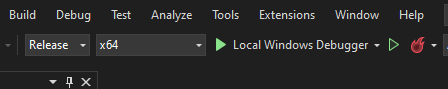
\includegraphics{../../../shared_latex_inputs/images/visual_studio_build_release.png}
        \caption{Visual Studio Build Mode}
    \end{figure}
    
    \item Build the projects in the following order: 
		\begin{itemize}	
			\item SNOPT\_build
 			\item snopt\_interface
			\item ALL\_BUILD
		\end{itemize}
    
    \begin{figure}[H]
        \centering
        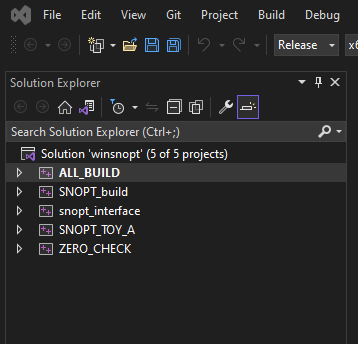
\includegraphics{../../../shared_latex_inputs/images/SNOPT_projects.png}
        \caption{Visual Studio SNOPT Solution Explorer}
    \end{figure}
    
    \item Verify the ouput window message says in part, ``0 failed, 0 skipped''. 
	The \verb|SNOPT\build\Release| directory should now look like the following image:
    
    \begin{figure}[H]
        \centering
        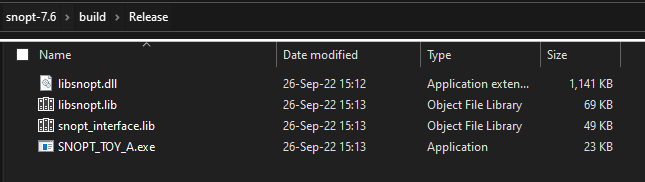
\includegraphics[width=0.9\textwidth]{../../../shared_latex_inputs/images/SNOPT_build_release.png}
        \caption{SNOPT Release Directory Contents}
    \end{figure}

\end{enumerate}
